\documentclass[11pt,en,number]{elegantpaper}
\newcommand{\upcite}[1]{\textsuperscript{\textsuperscript{\cite{#1}}}}
\usepackage{graphicx}
\usepackage{float}
\usepackage{subfigure}
\usepackage{changepage}
\title{Survey on Smart Customer Service}
\author{Muzhe Peng   2019124040}
\institute{CCNU-UOW JI}

 
\date{}

\begin{document}
\maketitle
\begin{abstract}
	Natural language processing (NLP) technology has always been considered a relatively mature branch of AI technology. However, although NLP does not perform well in an open domain environment, for limited scenarios, NLP and the knowledge map technology can show great value. Intelligent customer service is one of the most common applications of NLP and one of the most common applications of dialog systems. As an important part of enterprise customer relationship management (CRM), customer service is an important bridge between the enterprise and the customer, which greatly affects the company's sales results, brand influence and market position\cite{1}. However, for a long time, there have been many shortcomings in the customer service industry. The mobility of customer service personnel is high, the training costs are high, customer service is difficult to control, and a large number of repetitive problems consume excessive manual customer service. From the customer service data, it is found that business problems of enterprises are common problems faced by various types of enterprises. Because of these common problems, intelligent customer service came into being. 

	This paper mainly designs 3 usual Q\&A systems applied in smart customer service\cite{2}. IR (Information Retrieval) is mainly to find models and algorithms to obtain available information from the document set. The technical nature of the knowledge base question and answer is similar to the search engine technology, divided into two stages: the first stage is the recall of candidate collections, and the second stage is reordering. Reading comprehension uses machine reading comprehension technology to answer questions by reading and understanding unstructured articles to get answers. At the end of the paper, we talk about the evaluation standard of a Q\&A system and the possible future trend of smart customer service.
	% \keywords{Elegant\LaTeX{}, Working Paper, Template}
\end{abstract}
	
	
\section{Introduction}
	Traditional customer service mostly relies on humans to provide corresponding consulting and business services, and companies in various industries have a need for customer service personnel. In recent years, with the disappearance of the demographic dividend in China, the labor costs of various units have continued to increase, and due to the constraints of different professional levels and limited energy of customer service personnel, traditional customer service has gradually exposed weaknesses of low efficiency, low intelligence, and other issues.

	Due to the development of china's internet economy, business consulting channels have also changed from a single telephone consultation to multiple channels such as WeChat, Weibo, App, and web pages. Traditional customer service personnel have gradually become weaker in terms of time, energy, labor costs and so on.
	
	Customer service, as a booster for the development of corporate business, plays a vital role in the development of the company. In each period, it has relied on related technologies to promote the development and development of customer service software, laying the foundation for the intelligent development of customer service. From 1990 to 2000, the Internet had not yet gained popularity in China. At this time, the customer service software was mainly traditional call centers. From 2000 to 2010, with the popularization of the Internet in China, PC webpage online customer service and traditional customer service software were promoted simultaneously. After 2010, SaaS-based cloud call centers and cloud customer service software appeared, and customer service robots entered the commercial application stage. In recent years, with the improvement of the underlying AI technologies such as NLP technology, deep learning technology, and speech recognition technology, customer service software has gradually evolved toward intelligence\cite{3}.
	
	
\section{Problem Description}
	\subsection{Application in Real Enterprises}
	Enterprises have limited understanding of intelligent customer service robots. Intelligent robots use a large number of international cutting-edge technologies such as artificial intelligence, speech recognition, knowledge management, and human-computer interaction. They belong to a relatively professional field, and companies often do not know when they choose partners. How to choose and fail to formulate the correct measurement and screening standards leads to difficulties in practical applications, hinders the road of enterprise technology upgrade, and is a blow to the intelligent customer service industry\cite{4}.

	\subsection{Difficulties of mission robots}
	There are several difficulties for a mission robot in a single-round dialogue, one problem is that the same meaning may has different expression, it's difficult for a robot to precisely understand all these expressions. What's more, slight difference in even a single character can cause totally different meaning, even more, the same character could has different meaning. Last but not least, we need to cluster high-frequency problems, automatically learn to optimize the knowledge base\cite{5}.

\section{Overview of smart customer service}
	Intelligent customer service, which is what we call customer-maintained intelligent services, such as our common Taobao Xiaomi and JD.com.
	
	Currently limited by the level of NLP algorithm, intelligent customer service now plays a supporting role in actual use. At present, the most common form of intelligent customer service is to expand the function of intelligent customer service based on the manual customer service system. The most common functions are single round of question and answer, functional dialogue, and human-machine collaboration.
	
	Human-machine collaboration usually means that the intelligent customer service answers the questions first, and it cannot be transferred to manual labor, that is, the intelligent customer service solves certain high-frequency simple problems, and the difficult problems are transferred to the manual customer service.
	
	According to the common single-round question and answer of intelligent customer service, the technical essence of knowledge base question and answer is similar to the search engine technology, which are information retrieval\cite{6}.
	
	In fact, the intelligent customer service has undergone the following four stages of development:
	
    \begin{enumerate}
	  \item Accurate matching according to a single keyword: it can be defined as a mechanical customer service robot. It is similar to the keyword response in the WeChat official account background. A precise vocabulary can pop up a response. If there is a slight deviation, the customer cannot get the corresponding answer;
	  \item Fuzzy matching, keywords that meet similar meanings: based on the literal similarity of sentences, it performs fuzzy matching on a pre-defined Q\&A knowledge base to achieve answers to similar questions from different users. 
	  \item Natural language and semantic analysis to achieve more accurate answers to complex user inquiries: splitting a sentence, analyzing each word in it, adding a weight to each word, and matching the answers in the knowledge base according to a comprehensive algorithm of weights;
	  \item Deep learning, robots better understand human intentions: the most advanced machine learning algorithm currently , including recurrent neural networks, convolutional neural networks, LSTM (Long and Short Memory Networks), and so on. Deep learning algorithms can model the context, improve the semantic recognition ability, learn from a large amount of unlabeled data to understand the context, and then analyze the customer emotions in real time to give accurate answers. 
	\end{enumerate}
	\subsection{Intelligent customer service based on information retrieval}
	Information Retrieval(IR) is mainly to find models and algorithms to obtain available information from the document set. The user enters a query field that expresses demand information, and the system responds with a list of documents containing the required information. For example, we usually use Baidu, Google search.
	
	At present, most IR systems are based on an extreme version of combined semantics. The user's query content is expressed as the information requirements of the search term. The search term is processed for word disambiguation and synonym expansion (such as synonym expansion, which can be achieved through WordNet synonym set)\cite{7}. To generate the corresponding vector, the query vector and the document vector (the vectors of each other are weighted, such as TF-IDF) to calculate the similarity (can be calculated by cosine, the closer to 1 the more similar, the closer to 0 the more independent), as shown below.
	
	Among them, the document represents the text unit indexed by the system and provided for retrieval, the document list represents a set of documents used to meet the needs of the user, and the search term refers to a vocabulary item appearing in the document list, which can be used as an index.
	\begin{figure}[H]
		\centering
		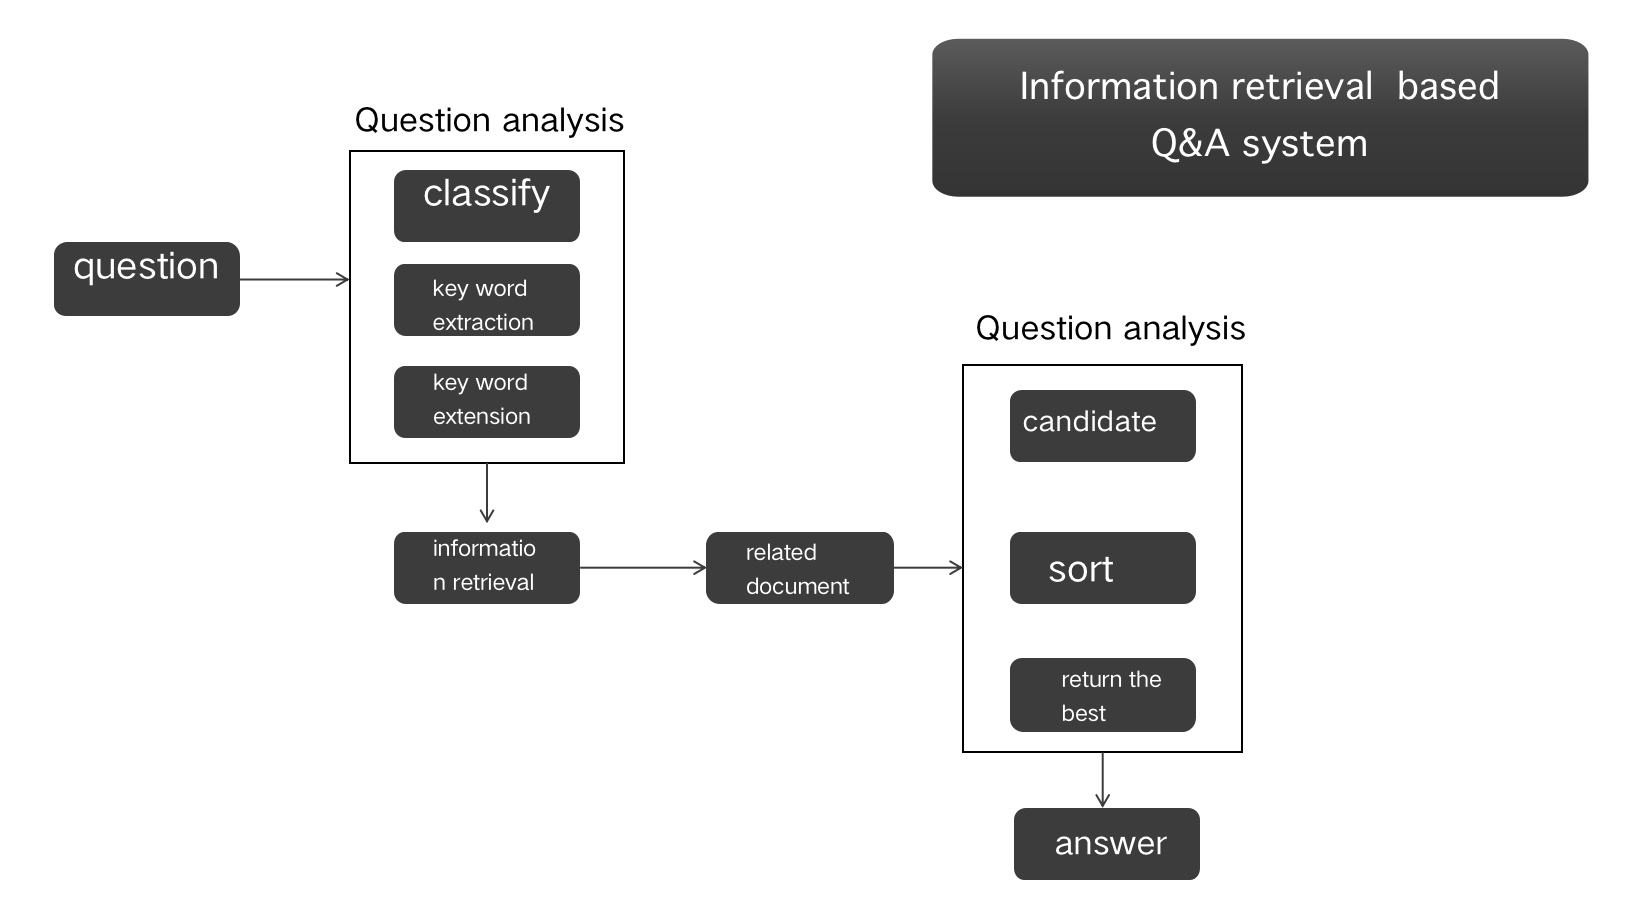
\includegraphics[width=13cm, height=8cm]{IR}
		\caption{Intelligent customer service based on information retrieval}
	\end{figure}
	In fact, the information retrieval architecture in the figure above returns a list of documents, and the intelligent customer service Q \& A returns the content of the answer. Let us look at the difference between Q \& A and information retrieval:
	\begin{figure}[H]
		\centering
		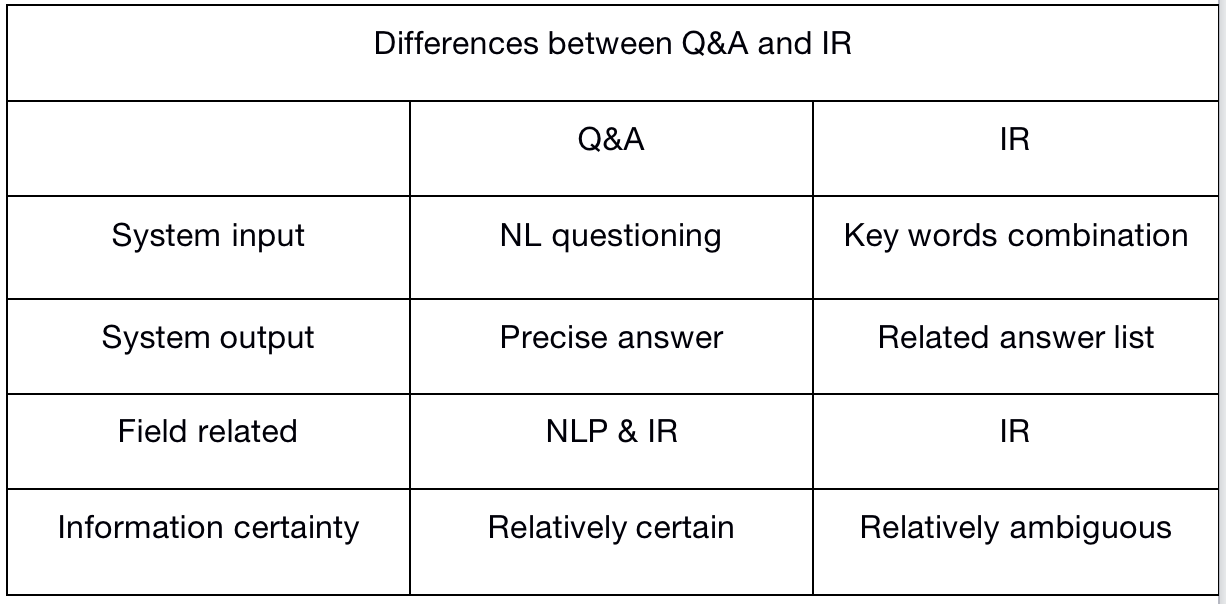
\includegraphics[width=11cm, height=5cm]{Differences}
		\caption{Differences between Q\&A and IR}
	\end{figure}
	We can see that Q \& A integrates technologies such as knowledge representation, information retrieval, natural language processing, and intelligent reasoning. After all, what the user wants is to obtain a specific piece of information, the answer to the question, and the required solution, such as how to reset the password of the user's question.
	
	At this time, we should return the solution to the user's problem to reset the password. Therefore, when the intelligent customer service's question and answer application information is retrieved, the corresponding adjustments are made. The answer returned is the answer, that is, the candidate answer with the highest probability of calculation. (Understand as a so-called recommendation). At the same time, when a problem query is processed, a problem classification module is added, that is, what type of question is, and the type can be answered better. The classifier can be trained by labeling the type of dialog data.
	
	\subsection{Intelligent customer service based on knowlege base}
	Now that we understand the implementation of the intelligent customer service model, if the dialogue system does not have a corpus, it will still not be able to talk, which is why so-called clever women can hardly do anything. The corpus is what we call the intelligent customer service. The knowledge base can come from the knowledge map or question and answer library we organize. The difficulty of the knowledge base lies in the cold start of the data, the cleaning and organization of the data.
	
	The cold start of the data, that is, whether there is any problem in generating the original data of the knowledge base (data cold start also affects the training of the information retrieval model), but the intelligent customer service is generally limited to the domain and applied to the service of its own enterprise. It is a manual service, so we can generally accumulate the data of artificial dialogue as the original data of the knowledge base (generally, the data in a certain period is selected, which is universal).
	
	Data cleaning and collation, that is, how to generate a complete and readable knowledge base after the original data. One of our common knowledge bases is the so-called question and answer library (that is, question-answer pairs, of course, there are usually other labels, such as manually labeled question types). The question and answer database is generated. We can use the original conversation data to the same identifier conversation (representing the complete conversation between the same user and the human customer service), and use the N-gram to splice the same ID segments according to the different conversation IDs (mainly by words The unigram, bigram, and trigram appearing in the bag are generally to trigram. Too few sentences are not smooth and too much calculation. After all, the size of the N-ary model is almost an exponential function of N, that is, $O (| V | ^ N)$, and V is a vocabulary\cite{8}. N-gram segments can be stitched together using the N-gram stitching algorithm, which can generally be processed by the NLTK toolkit) to become a smoother segment, and then manually reviewed and labeled to form a complete and readable Q \& A knowledge base.
	
	The bag of words refers to a piece of text (such as a sentence or a document) that can be represented by a bag containing these words. This representation does not take the grammar and the order of words into account; N-gram, which is N-gram grammar, refers to n consecutive words appearing in the text. The N-gram model is a probabilistic language model based on the (n-1) - order Markov chain. The next word is predicted from the n-1 words that appear before. The probability of the appearance of n words to infer the structure of the sentence; when n is 1, 2, 3, they are also called unigram, bigram, and trigram.
	
	The following figure is an example of the question and answer library in the above dialogue, after being processed by N-gram stitching, and then manually reviewed and marked:
	\begin{figure}[H]
		\centering
		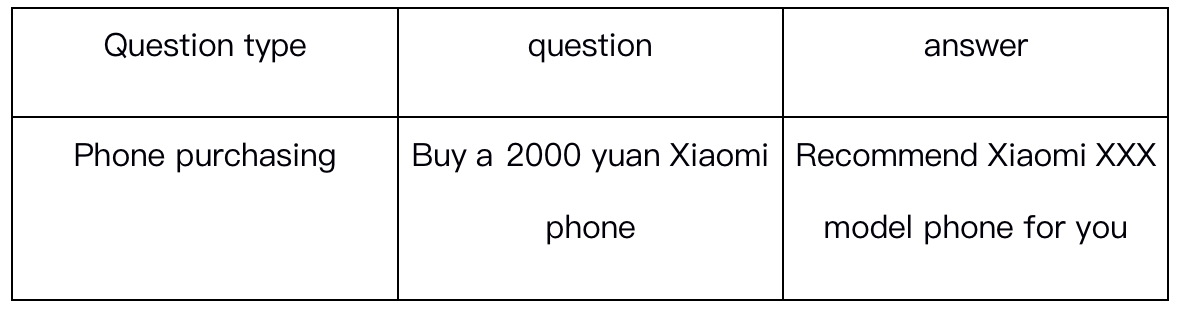
\includegraphics[width=12cm, height=3cm]{KB}
		\caption{Example of the question and answer library}
	\end{figure}
	However, due to the singularity of questions in the Q \& A library, when users use similar questions to ask questions, users may be dissatisfied because there is no corresponding answer to questions such as models. Even if we generalize the problem, such as extending the problem, using the slack mode allows matching the results of ignoring part of the text, but it will cause some incorrect results and also cause user dissatisfaction. Therefore, in order to improve the accuracy of the question, we can use the seed mode, that is, use the keyword of the organized knowledge base to search on the original or cleaned conversation data set, check the common questions of users, and expand the question and answer. Add similar questions to the question, such as the question in the question and answer library above, "buy a 2000 yuan Xiaomi phone", and expand the similar question "recommend a 2000 yuan mobile phone, no limit to the brand."
	
	Of course, the richer the knowledge base, the better. After all, the richer the knowledge, the broader the scope of business issues covered, and the better the availability of solving user needs. The broader the knowledge, as we humans, can solve more problems, the better our ability.
	\subsection{Q \& A system based on reading comprehension}
	It uses machine reading comprehension technology to answer questions by reading and understanding unstructured articles to get answers, and it can be divided into extractive Q\&A and generative Q\&A\cite{9}.
	\begin{figure}[H]
		\centering
		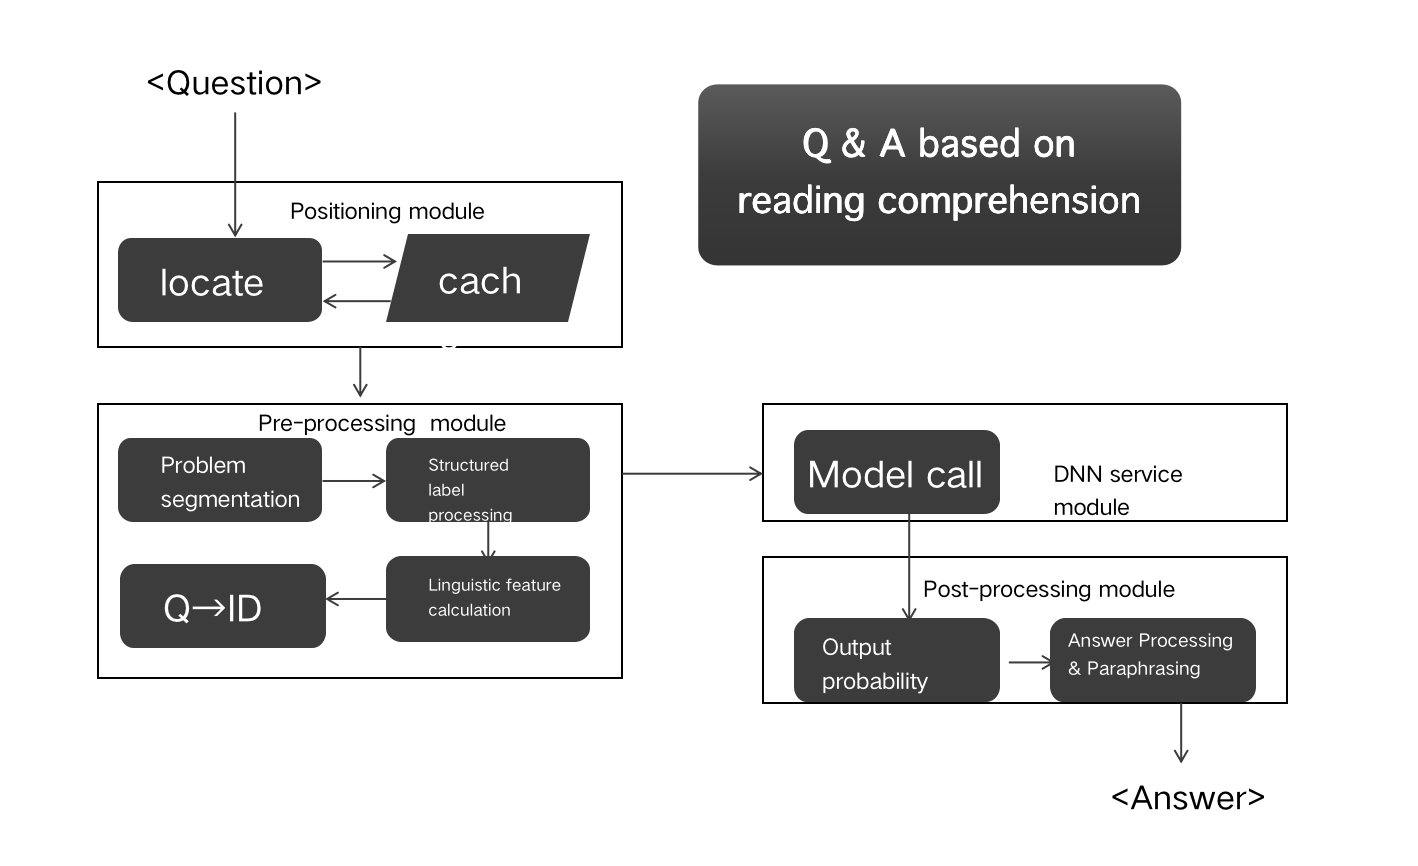
\includegraphics[width=13cm, height=8cm]{RC}
		\caption{Q \& A system based on reading comprehension}
	\end{figure}
	Extractive QA system
	
	Extractive QA allows users to enter several unstructured texts and several questions. Based on reading comprehension, the machine automatically finds answers in the text to answer user questions. The answer to a question in extractive QA must appear in an article\cite{10}.
	The classic data set of extractive Q\&A is SQuAD (Stanford Question and Answer Data Set), which is a reading comprehension data set composed of crowdsourced staff based on a series of Wikipedia articles' questions and corresponding answers, the answers to each question are relevant A snippet or section of text in an article. SQuAD has a total of 107,785 questions and accompanying 536 articles.
	
	Generative QA system
	
	Generative QA answers have the following form\cite{11}:
	The answer lies entirely in the original text:
	\begin{itemize}
		\item The answers appear in multiple articles, respectively;
		\item Part of the answer appears in the original text, and part of the answer appears in the question;
		\item Part of the answer appears in the original text, and the other part is the generated new word;
		\item The answer does not appear at all (Yes / No type);
	\end{itemize}

	The current better dataset is MS MARCO from MSRA. For this data set, domestic Baidu and Ape Question Bank have given their own evaluation.
	\section{Design and Evaluation}
		Intelligent customer service is not an open chat dialogue system, but a dialogue system based on specific business areas and business scenarios. The purpose is to quickly solve the needs of users. An ideal dialogue system is a system that can help users achieve their goals with minimal cost\cite{12}. Therefore, intelligent customer service should be a user-centric design principle, and user satisfaction is of paramount importance.
		\subsection{Design}
		Due to its own purpose, the intelligent customer service should select the corresponding design principles such as dialogue strategies, prompts, and error information feedback according to its own business scenario.
		
		Common design points\cite{13}:
		\begin{itemize}
		\item Research users and businesses: analyze user portraits, research common problems of users, learn potential problems of users, recommend and guide them accordingly, and personally answer users; for example, each user enters the intelligent customer service, and the problem guidance of the interface is different;
		
		\item Dialogue strategy: Questions with high similarity are feedback answers, and some similar questions can be fed back to similar questions. Convergence guides users to ask questions. Convergence guides users to ask questions, and guides users to re-question or direct manual customer service. At the same time, a chat library is added to ensure users The smoothness of the conversation prevents some users from chatting and not responding. Of course, there is also rapid convergence. When a user enters a message through a Lenovo question display to prompt the user to choose a question, there is also a strategy of universal instructions, which can be used anywhere in the dialog so that users can request corresponding operations, such as our common universal Instructions: Help (return to the help menu), manual or manual customer service (transfer to manual customer service);
		
		\item Integrity of dialogue data: After the user transfers to the manual customer service, the data of the user and the system are transferred to the manual customer service dialogue window at the same time. Increase user satisfaction;
		Iterative design: data monitoring, analysis and optimization based on index data; optimization based on user satisfaction opinions; maintenance and update of knowledge base (including model independent learning).
		\end{itemize}
		\subsection{Evaluation}
		User satisfaction is the measure of our intelligent customer service. Users can give explicit feedback on the system interface satisfaction questionnaire. This is the true evaluation of the users we get directly. However, feedback on user satisfaction requires operating costs after all, and many users will not respond. Therefore, we have fewer direct satisfaction evaluations, and more often use other measurement indicators for a comprehensive evaluation system.
		Evaluation generally includes external and internal evaluation indicators. External indicators refer to some indicators that are visible to our business, such as intelligent customer service problem resolution rates, manual customer service system connection rates or session duration, and other measurement indicators. Some indicators of the model algorithm, common evaluation indicators of information retrieval: precision, recall, F-measure value. Appropriate evaluation indicators can be selected according to specific business scenarios.
	\section{Conclusion}
	In recent years, China's CPI has been increasing year by year, which has promoted the rise in labor costs. Consequently, reducing staff and increasing efficiency has become the consensus of business operations, especially for traditional customer service centers which has been considered as cost centers. In the future, The gradually mature intelligent customer service robots may become more popular.

	Currently limited by the level of NLP algorithm, intelligent customer service is currently more assisted by manual customer service\cite{14}. In the future, if you want to further replace manual customer service, NLP technology should be able to achieve better multi-round conversation modeling and personalized responses to understand the user ’s True intentions and dialogue are natural.

	After all, for intelligent customer service, the important premise is to accurately understand the user's problem, and at the same time, you can contact the context, conduct natural multiple rounds of dialogue with the user, understand the user's intention, and solve the user's problem.

	\nocite{*}
\bibliography{ref}

\end{document}
